\documentclass[subscriptcorrection,upint,varvw,barcolor=Goldenrod3,mathalfa=cal=euler,balance,hyphenate,french,pdf-a]{asmejour}

\def\versionno{0.2} % Fix for pdflatex (file txmiaX): Font txmiaX at 342 not found

\hypersetup{
	pdfauthor={Sesha Charla},                       	   	% <=== change to YOUR name[s]!
	pdftitle={Modelling and Parameter Estimation of Diesel Engine Aftertreatment System under Catalyst Saturation
	for Aging Diagnostics},                  	% <=== change to YOUR pdf file title
	pdfkeywords={Diesel Engine Aftertreatment Systems, Diagnostics, Modelling, Nonlinear Systems, System Identification, Hypothesis Testing, Statistical Detection},% <=== change to YOUR pdf keywords
	pdfsubject = {Mathematical Modelling, Identification and Diagnostics},			% <=== change to YOUR subject
}


\JourName{Dynamic Systems, Measurement, and Control }%<=== change to the name of your journal

\PaperYear{2026}

% Custom Stuff
%% === INLINED from: ltx_core/ltx_pkgs.tex ===
% \usepackage{amsmath}  % loaded by asmejour.cls
\setcounter{MaxMatrixCols}{20}
% \usepackage{mathtools}  % loaded by asmejour.cls
% \usepackage{amssymb}
\usepackage{float}
% \usepackage{graphicx}  % loaded by asmejour.cls
\usepackage{caption}
\usepackage{extarrows}
% \usepackage{xcolor}  % loaded by asmejour.cls
\usepackage{lscape}
\usepackage{pdflscape}
\usepackage{pdfpages}
\usepackage{multicol}
\usepackage{leftindex}
\usepackage{nicefrac, xfrac}
\usepackage{algorithm2e}
\SetKwComment{Comment}{/*}{*/}
% \usepackage{mathtools}  % loaded by asmejour.cls (duplicate)
% \usepackage{hyperref}
\hypersetup{ colorlinks=false }
\usepackage{asmewide}
\usepackage{paralist}
\usepackage{fancybox,framed}
\usepackage{indentfirst}
\usepackage[T1]{fontenc}
\usepackage{graphics} % for pdf, bitmapped graphics files
\usepackage{epsfig} % for postscript graphics files
% \usepackage{mathptmx} % assumes new font selection scheme installed
% \usepackage{times} % assumes new font selection scheme installed

% Listings
\usepackage{listings}
% \usepackage{color}  % xcolor already loaded by asmejour.cls
%% === INLINED from: ./ltx_core/lst_style.tex ===
\definecolor{mygreen}{rgb}{0,0.6,0}
\definecolor{mygray}{rgb}{0.5,0.5,0.5}
\definecolor{mymauve}{rgb}{0.58,0,0.82}

\lstset{
  backgroundcolor=\color{white},   % choose the background color; you must add \usepackage{color} or \usepackage{xcolor}; should come as last argument
  basicstyle=\small\ttfamily,        % the size of the fonts that are used for the code
  breakatwhitespace=false,         % sets if automatic breaks should only happen at whitespace
  breaklines=true,                 % sets automatic line breaking
  captionpos=t,                    % sets the caption-position to bottom
  commentstyle=\color{mygreen},    % comment style
  deletekeywords={...},            % if you want to delete keywords from the given language
  escapeinside={\%*}{*)},          % if you want to add LaTeX within your code
  extendedchars=true,              % lets you use non-ASCII characters; for 8-bits encodings only, does not work with UTF-8
  firstnumber=1,                % start line enumeration with line 1000
  frame=false,	                   % adds a frame around the code
  keepspaces=true,                 % keeps spaces in text, useful for keeping indentation of code (possibly needs columns=flexible)
  keywordstyle=\color{blue},       % keyword style
  language=Python,                 % the language of the code
  morekeywords={*,...},            % if you want to add more keywords to the set
  numbers=none,                    % where to put the line-numbers; possible values are (none, left, right)
  numbersep=5pt,                   % how far the line-numbers are from the code
  numberstyle=\tiny\color{mygray}, % the style that is used for the line-numbers
  rulecolor=\color{black},         % if not set, the frame-color may be changed on line-breaks within not-black text (e.g. comments (green here))
  showspaces=false,                % show spaces everywhere adding particular underscores; it overrides 'showstringspaces'
  showstringspaces=false,          % underline spaces within strings only
  showtabs=false,                  % show tabs within strings adding particular underscores
  stepnumber=5,                    % the step between two line-numbers. If it's 1, each line will be numbered
  stringstyle=\color{mymauve},     % string literal style
  tabsize=4,	                   % sets default tabsize to 2 spaces
  title=\lstname                   % show the filename of files included with \lstinputlisting; also try caption instead of title
}
%% === END of: ./ltx_core/lst_style.tex ===


% bibliography
\usepackage[utf8]{inputenc}
% \usepackage[english]{babel}  % Already loaded by asmejour class

% \usepackage{biblatex}

% DOC compatible pdfs
\ifx\pdfgentounicode\undefined
\else
  \input{glyphtounicode}
  \pdfgentounicode=1
\fi
%% === END of: ltx_core/ltx_pkgs.tex ===
%% === INLINED from: ltx_core/new_cmds.tex ===
% NewCommands
\newcommand{\peq}{ \mathrel{+}= }
\newcommand{\muleq}{ \mathrel{*}= }
\newcommand{\sign}{ \text{sign}}
\renewcommand{\bm}[1]{\begin{bmatrix} #1 \end{bmatrix}}
\newcommand{\mat}[1]{\begin{matrix} #1 \end{matrix}}
\newcommand{\lx}[2]{\leftindex #1 {#2}}
\newcommand{\norm}[1]{\left\lVert #1 \right\rVert}
\newcommand{\itbf}[1]{\noindent\textit{\textbf{#1}}}
\newcommand{\mdet}[1]{\norm{\begin{matrix} #1 \end{matrix}}}
\newcommand{\pbox}[1]{\fbox{\begin{minipage}{\textwidth} #1 \end{minipage}}}
\newcommand{\lstln}[1]{\lstinline|#1|}
\newcommand{\lr}[1]{\left( #1 \right)}
\newcommand{\lrb}[1]{\left[ #1 \right]}
\newcommand{\lrf}[1]{\left\{ #1 \right\}}
\newcommand{\adj}{\text{adj}}
\newcommand{\mol}[1]{\lrf{#1}}
\newcommand{\con}[1]{\lrb{#1}}
\newcommand{\abs}[1]{\left\lvert #1 \right\rvert}
\newcommand{\sat}{\text{sat}}
\newcommand{\kron}{\otimes}
\newcommand{\Var}{\text{Var}}
\newcommand{\froot}{.} % Root director for the files
\newcommand{\figWidth}{0.45\textwidth}
\DeclareMathOperator*{\argmax}{arg\,max}
\DeclareMathOperator*{\argmin}{arg\,min}
%%=== Lemmas and Theorems
\newtheorem{theorem}{Theorem}
\newtheorem{corollary}{Corollary}[theorem]
\newtheorem{lemma}[theorem]{Lemma}

%% Chemcial Formulae in MathMode
\newcommand{\nox}{\text{NO}_{\text{x}}}
\newcommand{\ammonia}{\text{NH}_{3}}
\newcommand{\oxygen}{\text{O}_{2}}
\newcommand{\water}{\text{H}_{2}\text{O}}
\newcommand{\nitrogen}{\text{N}_{2}}
%% === END of: ltx_core/new_cmds.tex ===

\PreprintString{}

\begin{document}
%=======================================================================================================================
\SetAuthorBlock{Sesha Charla}{School of Mechanical Engineering,\\
   Purdue University,\\
   West Lafayette, Indiana, USA\\
   email: scharla@purdue.edu}

\SetAuthorBlock{Peter H. Meckl\CorrespondingAuthor}{%
   Fellow ASME\\
   School of Mechanical Engineering,\\
   Purdue University,\\
   West Lafayette, Indiana, USA\\
   email: meckl@purdue.edu
}

\SetAuthorBlock{Bin Yao}{%
   Fellow ASME\\
   School of Mechanical Engineering,\\
   Purdue University,\\
   West Lafayette, Indiana, USA\\
   email: byao@purdue.edu
}
%=======================================================================================================================
\title{Modelling and Parameter Estimation of Diesel Engine Aftertreatment System under Catalyst Saturation for Aging
   Diagnostics}

\keywords{Diesel Engine Aftertreatment System, System Identification, Switched Nonlinear Systems, Parameter Estimation, Convex Optimization, Statistical Estimation and Detection.}

%=======================================================================================================================
%% Abstract should be no more than 250 words
\begin{abstract}
%% === INLINED from: secs/0-abstract.tex ===
This paper presents a model-based statistical framework for detecting catalyst aging
in diesel engine SCR systems. A dynamic model for $\nox$ reduction under catalyst
saturation with ammonia is derived from molar conservation, accounting for the
interplay between residence time and sensor sampling frequency. The model parameters
are estimated via maximum likelihood using the bounding relationship between actual
and predicted $\nox$ reduction under saturation while handling uncertainties from
$\nox$ sensor cross-sensitivity in the absence of ammonia sensors. The estimated
parameters are shown to be sensitive to the catalyst's aging state, enabling a Wald
test-based hypothesis-testing framework for aging detection. The proposed detector is
validated using test-cell data at different aging levels and real-world data from four
long-haul trucks.
%% === END of: secs/0-abstract.tex ===
\end{abstract}

%=======================================================================================================================
\date{Version \versionno , \today}
\maketitle
%=======================================================================================================================

%% === INLINED from: secs/1-intro.tex ===
\section{ Introduction }
%===
Diesel engine aftertreatment systems reduce the concentrations of harmful gases such as $\nox$ and $\text{CO}$ from
exhaust emissions. The Selective Catalytic Reduction (SCR) system reduces the engine-out $\nox$ to $\nitrogen$ and
$\water$ using ammonia from urea dosing in the presence of a catalyst. This catalytic conversion process is regulated to
decrease the levels of ammonia in the exhaust (ammonia slip) via two methods. The first is feedback control, which
adjusts the urea injection rate based on the exhaust $\nox$ concentrations. The second method involves an additional
catalytic reaction, the Ammonia Slip Catalyst (ASC), which is designed to oxidize any excess ammonia at the end of the
SCR bed. Figure-\ref{fig:exhaust_scheme} shows a schematic of the SCR-ASC system. It has been found that the
$\nox$-reduction capacity of the catalyst decreases over time due to hydrothermal aging and deposition of contaminants
such as excess urea, platinum, sulfur and phosphorus \cite{matsumoto2016model}. The aging of the catalyst leads to
increased emissions of $\nox$ and ammonia slip, which can result in non-compliance with environmental regulations. A
fault detection system for catalyst aging would provide better control over system maintenance and improve the overall
reduction in emissions.

\begin{figure}[ht]
    \centering
%%     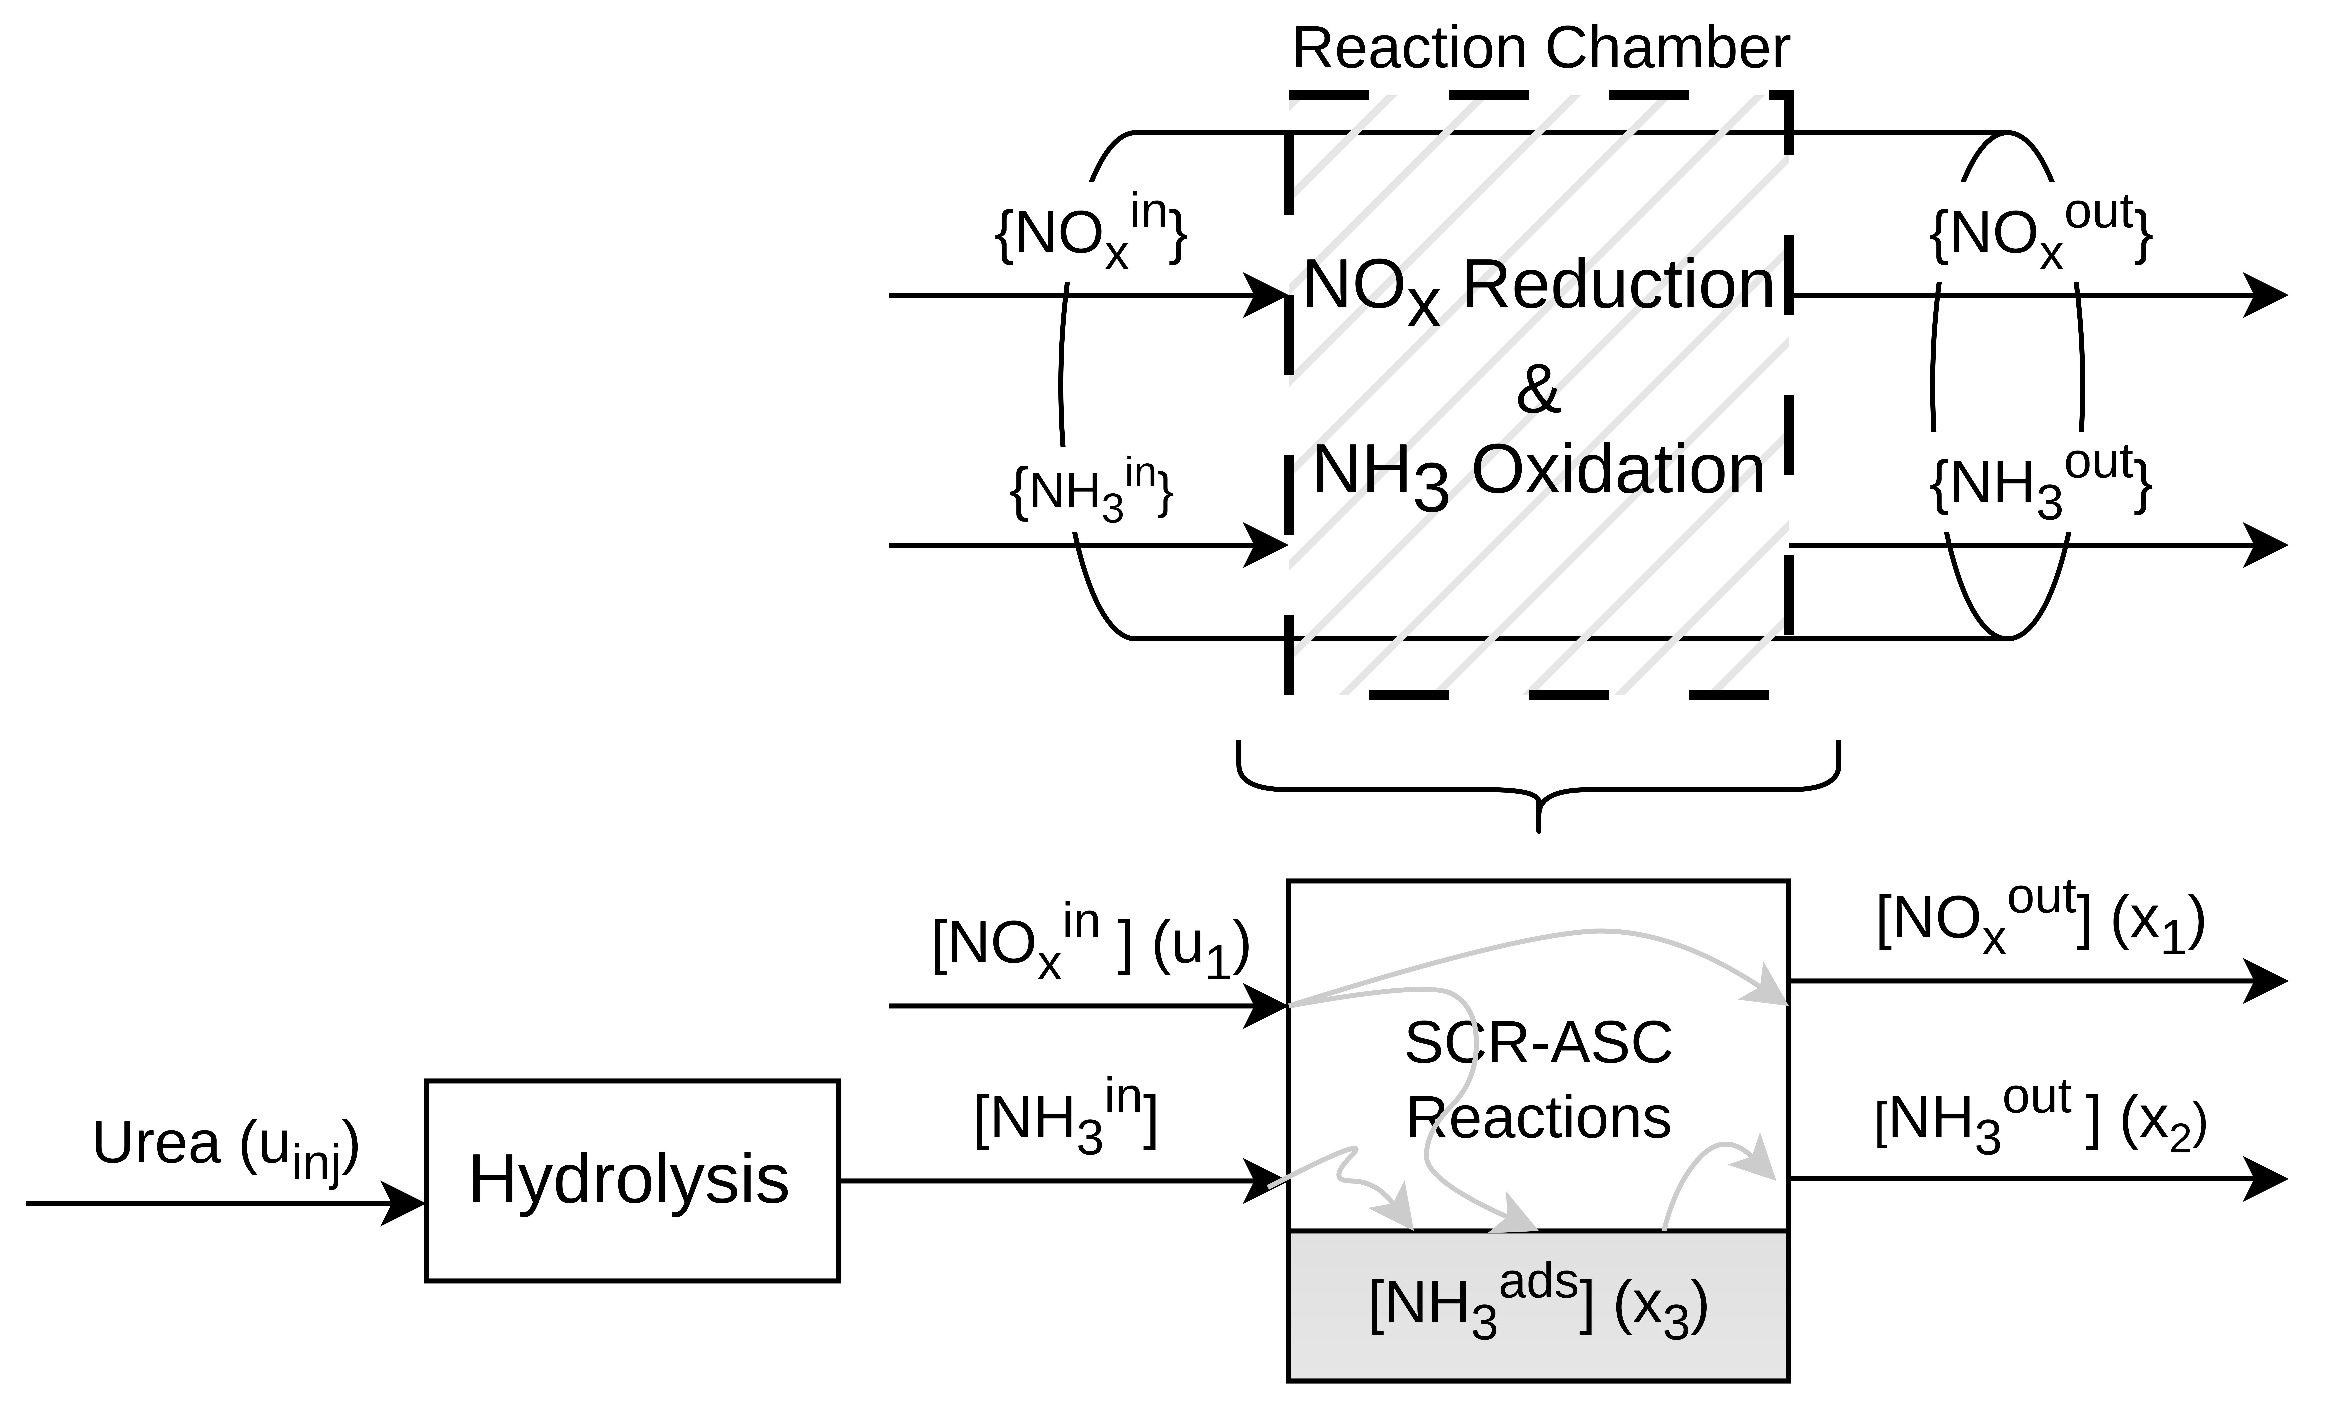
\includegraphics[width=0.45\textwidth]{./figs/1_intro/fig1_SCR-ASC_ModelReduction.eps}
    \caption{Schematic of the SCR-ASC system}
    \label{fig:exhaust_scheme}
\end{figure}

Thus, modern diesel aftertreatment systems, particularly those that integrate Selective Catalytic Reduction (SCR) with
Ammonia Slip Catalyst (ASC), necessitate advanced onboard diagnostics (OBD) tools for accurate assessment of catalyst
aging. However, the effectiveness of traditional OBD approaches for this purpose has been impeded by the absence of
model validation with real-world catalyst degradation data, the limitations imposed by existing commercial $\nox$
sensors' cross-sensitivity to ammonia, and the absence of ammonia sensors in commercial vehicles.

Numerous studies have been conducted on modeling SCR-ASC systems and their control \cite{yuan2015diesel}. A prevalent
modeling approach is to approximate the PDE model for the plug flow reaction as a set of ODEs using a sequence of
Continuously Stirred Tank Reactors (CSTRs) (\cite{hsieh2011development} , and \cite{nova2014urea}). The
single CSTR approach was first justified in \cite{devarakonda2008adequacy} and a nonlinear model was developed using
these assumptions, which was then linearized for feedback control design (\cite{devarakonda2009model}). With this model,
observers were designed to estimate the states corresponding to the catalyst's storage (\cite{ma2017observer},
\cite{jain2020term}). A method for detecting the catalyst's aging using an observer for the change in the maximum
storage capacity of the catalyst, modeled as an exponential function of temperature, was also proposed in
\cite{ma2017observer} and \cite{jiang2019hydrothermal}. Alternatively, an onboard diagnostics (OBD) logic for catalyst
aging based on the tailpipe $\nox$ and ammonia is proposed in \cite{matsumoto2016model} based on the hypothesis of
reduction in adsorption sites and demonstrated on real-world trucks. A common theme in these studies is that the system
identification results in a non-convex, nonlinear parameter estimation problem. Moreover, these studies assume the
availability of all the gaseous states at the tailpipe for state estimation and to eliminate the effects of
cross-sensitivity of the $\nox$ sensors, which is not always the case in real-world applications as tailpipe ammonia
measurements are not generally available in commercial vehicles. Another fundamental issue with the CSTR model in the
context of sensor sampling is that the discretization of the continuous model does not account for the residence time
of the reactants \cite{charla2026board}, resulting in high sampling frequency requirements that are not feasible in
practice. Additionally, the discretization requires at least two CSTRs to capture the system dynamics and causality
\cite{charla2024reduced}, thereby increasing the model order.

An alternative approach to the problem would be discarding the CSTR assumption and modelling the time evolution of the
sensor signals when a "plug" or "parcel" of the exhaust gases flows through the chamber in discrete time, considering
the interplay between sampling and residence time of the reactants. The catalyst saturation that is inherently
considered in the CSTR approach needs to be explicitly included as a separate mode of the system.

This work develops such a nonlinear model for $\nox$ reduction under catalyst saturation, which serves as one of
the modes within a complete switched nonlinear framework. Following the model development, we present an algorithm to
estimate the parameters of the saturated catalyst model using real-world data. This estimation explicitly accounts for
unknown operating modes, uncertainties arising from $\nox$ sensor cross-sensitivity to ammonia, and the absence of
dedicated ammonia sensors. Utilizing these estimates, we introduce a catalyst mode detection algorithm to characterize
the statistical properties of the parameter estimates. The limitations of both the estimation method and this mode
detection approach are discussed and demonstrated in the appendix. Finally, we develop a statistical test for detecting
catalyst aging based on these estimated parameters, with its performance demonstrated using both test-cell and
real-world truck data.
%% === END of: secs/1-intro.tex ===
%% === INLINED from: secs/2-SatSys_model.tex ===
\section{SCR-ASC System Dynamics Under Catalyst Saturation}
%==
The SCR-ASC subsystem in the diesel engine aftertreatment systems involves reacting flow over a catalyst that
adsorbs ammonia from urea decomposition. The reaction kinetics start with the decomposition of urea into ammonia
followed by its adsorption onto the surface of the catalyst. The $\nox$ entering the chamber is reduced by this adsorbed
ammonia. The Eley-Rideal reaction mechanism \cite{prins2018eley}, \cite{yuan2015diesel}, \cite{hsieh2011development},
\cite{nova2014urea} is considered for modeling the SCR reaction kinetics, where one reactant is in the gas phase ($\nox$), and
the other is adsorbed on the catalyst surface $(\ammonia)$. Reference~\cite{nova2014urea} lists all the reactions that take place
inside the SCR-ASC chamber. Ammonia oxidation (AMOX) happens on the surfaces of both the SCR and the ASC
catalysts, but the SCR catalyst favors $\nox$ reduction while the ASC is specifically designed for ammonia oxidation.
In order to keep the model order reasonably low and parameters identifiable, only the following three prominent reactions \cite{devarakonda2008adequacy},\cite{hsieh2011development} are considered:
\begin{enumerate}
    \item Standard SCR reaction:
    \begin{align}
        4 \ammonia ^{ads} + 4 \text{NO} + \oxygen &\xrightarrow[]{k_{scr}} 4 \nitrogen + 6 \water \label{eqn::std_scr}
    \end{align}
    \item Ammonia Oxidation:
    \begin{align}
        4 \ammonia^{ads} + 3 \oxygen &\xrightarrow[]{k_{oxi}} 2 \nitrogen + 6 \water \label{eqn::amox}
    \end{align}
    \item Ammonia Adsorption/Desorption:
        \begin{align}
            \ammonia + \Theta_{free} &\xrightleftharpoons[k_{des}]{k_{ads}} \ammonia^{ads}
            \label{eqn::ads}
        \end{align}
\end{enumerate}
%==
This aggregation of reactions results in errors in parameter estimates; specifically, parameters containing the rate
constant for the $\nox$ reduction $\lr{k_{scr}}$ have higher (bounded) uncertainty because they become dependent on the
nitrogen selectivity of the AMOX reaction \cite{jain2023diagnostics}.
%=======================================================================================================================
\begin{figure}[ht]
    \centering
%%     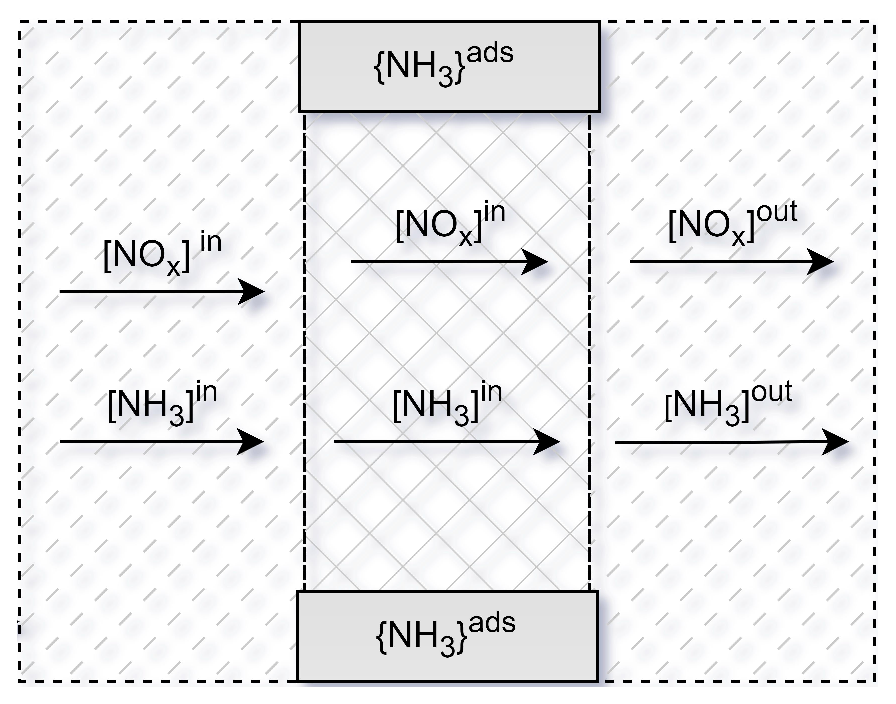
\includegraphics[width=0.3\textwidth]{figs/2_mdl/fig2_plug_flow_discrete.eps}
    \caption{Control volume in plug flow reaction}
    \label{fig:plug-flow}
\end{figure}
%===
%% === INLINED from: secs/2-subs/2-0-sat_NOx_deriv.tex ===
%% 1. The \nox reduction dynamics are different when the catalyst is saturated as it is independent of the urea-dosing.
%====
Considering the reaction chamber as a control volume (Figure-\ref{fig:plug-flow}), the dynamic model is developed based
on the molar conservation of species at the inlet and outlet separated by a residence-time interval. By assuming a
zero-order hold on the inlet species over the sampling time, the equations relating inlet and outlet concentrations at
the residence-time scale are extended to the sampling-time scale. The residence time can be parameterized as a function of mass flow rate $\lr{F}$ assuming that the effect of the density variation on residence time is insignificant:
\begin{align}
        \tau(k) & = \frac{\rho V_{scr}}{F(k)} = \frac{\tau_0}{F(k)}
        \label{eqn::res_time}
\end{align}
Let $\lrf{\bullet}$ be the number of moles and $\lrb{\bullet}$ be the concentration of a given species $\bullet$. We have the molar conservation of $\nox$ across the control volume $(V_{scr})$ within one residence time $(\tau)$:
%====
\begin{multline}
        \mol{\nox}^{out} (t + (i+1) \tau) =
        \mol{\nox}^{in} (t + i \tau) \\
        + V_{scr} \int_0^{\tau} \frac{d}{dt} \con{\nox}^{scr}dt
        \label{eqn::nox_bal}
\end{multline}
%===
The number of moles entering at the inlet and leaving at the outlet can be written as a function of the concentration, residence time, and mass flow rate $(F)$:
%===
\begin{align}
        \mol{\nox}^{in/out} = \con{\nox}^{in/out} \tau \lr{\frac{F}{\rho}} = \con{\nox}^{in/out} V_{scr}
\end{align}
%===
Using the Eley-Rideal mechanism for the standard SCR reaction (\ref{eqn::std_scr}):
\begin{align}
        \frac{d}{dt} \con{\nox}^{scr}dt = -k_{scr} \con{\ammonia}^{ads} \con{\nox}^{in}
\end{align}
%===
Rewriting (\ref{eqn::nox_bal}) in terms of concentrations and integrating over the residence time:
\begin{multline}
        \con{\nox}^{out} (t + (i+1) \tau) =
        \con{\nox}^{in} (t + i \tau) \\
        -\tau k_{scr} \con{\ammonia}^{ads} \con{\nox}^{in}
        \label{eqn::nox_bal_con}
\end{multline}
%====
Summing the equations from (\ref{eqn::nox_bal_con}) for  $i = 0$ to $n-1$, where $n$ is the total number of residence
times within one sampling period $(n= t_s/\tau)$ and using the zero-order hold assumptions at the inlet
(\ref{eqn::zero_in}) and outlet (\ref{eqn::zero_out}) concentrations, we obtain (\ref{eqn::nox_avg}).
%===
\begin{align}
        \con{\nox}^{in} (t + i \tau)      & = \con{\nox}^{in}(t) \quad \forall i \in [0, n-1]  \label{eqn::zero_in}        \\
        \con{\nox}^{out} (t + (i+1) \tau) & = \con{\nox}^{out}(t + t_s) \quad \forall i \in [0, n-1] \label{eqn::zero_out}
\end{align}
%===
Letting tailpipe $\nox$ concentration be $x_1(k+1) = \con{\nox}^{out}(t+t_s)$ and inlet $\nox$ concentration be $u_1(k) = \con{\nox}^{in}(t)$, we get,
%===
\begin{multline}
        \underbrace{\con{\nox}^{out}(t+t_s)}_{x_1(k+1)} = \underbrace{\con{\nox}^{in}(t)}_{u_1(k)} \\
        - \tau(t) k_{scr}(t) \con{\nox}^{in}(t) \underbrace{\lrf{\frac{1}{n} \sum_{i = 0}^{n-1} \con{\ammonia}^{ads}(t + i \tau)}}_{\gamma(k)}
        \label{eqn::nox_avg}
\end{multline}
%
% ======================================================================================================================
%
The quantity $\gamma(k)$ is the average concentration of ammonia adsorbed on the catalyst's surface across the $n$ residence times between $k$ and $k+1$ samples. $\gamma(k)$ is bounded by the total concentration of voids on the surface of the catalyst, $\Gamma$, which decreases with increasing temperature.
\begin{align}
        0 \leq \gamma(k) \leq \Gamma \qquad \forall k
\end{align}
%===
The unbounded dynamics of $\gamma$, $\gamma^{ub}(k)$ are a nonlinear function dependent on the concentration of adsorbed ammonia, urea dosing $\lr{u_{inj}}$, and the inlet $\nox$ concentration from the previous time step \cite{charla2026board}.
\begin{align}
        \gamma^{ub}(k) & = g_{\gamma} \lr{ \gamma(k-1), u_{inj}(k-1), \con{\nox}^{in}(k-1) }
\end{align}
The actual expression, which is beyond the scope of this work, can be derived using a similar approach to that used to derive
$\nox$ process dynamics (\ref{eqn::nox_avg}). $\gamma(k)$ can be described using the following piecewise
function:
\begin{align}
        \gamma(k) & =
        \begin{cases}
                \gamma^{ub}(k) & \text{if } \quad 0 \leq \gamma^{ub}(k) \leq \Gamma                  \\
                \Gamma         & \text{if } \quad \gamma^{ub}(k) > \Gamma \qquad \text{[Saturation]} \\
                0              & \text{if } \quad \gamma^{ub}(k) < 0 \qquad \text{[Empty]}
        \end{cases}
\end{align}
%===
Let $\eta(k)$ be the $\nox$ reduction during a given time step $k$,
\begin{align}
        \eta (k+1) & = u_1(k) - x_1(k+1)
\end{align}
Introducing the above definition and the residence time expression (\ref{eqn::res_time}) into the $\nox$ process dynamics model (\ref{eqn::nox_avg}), we get,
\begin{align}
        \eta (k+1) & =   \frac{u_1(k)}{F(k)} \tau_0 \; k_{scr}(T(k)) \; \gamma (T(k)) \label{eqn::flow_scaled_nox_eff}
\end{align}
%===
For $\nox$ process dynamics under catalyst saturation, $\gamma(k) = \Gamma$.
\begin{align}
        \implies \eta_{sat} (k+1) & =  \frac{u_1(k)}{F(k)} \tau_0 \; k_{scr}(T(k)) \; \Gamma (T(k))
        \label{eqn::nox_mdl}
\end{align}
%===
The above equation~(\ref{eqn::nox_mdl}) shows that the tailpipe $\nox$ concentration becomes independent of urea dosing under catalyst saturation. Polynomial approximations of Arrhenius temperature dependence of the rate constant, $k_{scr}$ and the concentration of viable voids, $\Gamma$ (\cite{nova2014urea},\cite{ciardelli2004scr},\cite{joo2008study}), are used to get a linear-in-parameters model for the $\nox$ process dynamics.
\begin{align}
        k_{scr}(T) & = A_{scr} e^{\lr{-\frac{E_{scr}}{RT}}} \approx \sum k_i T^i  \qquad i = 0, 1, \hdots
        \label{eqn::rate_const}                                                                           \\
        \Gamma(T)  & = S_1 e^{-S_2 T} \approx \sum r_i T^i \qquad i = 0, 1, \hdots
        \label{eqn::gamma}
\end{align}
%===
The above approximate models for temperature dependence introduce parameter estimates that depend on temperature ranges
in the samples. For numerical stability \cite{press2003numerical}, the given temperature range is mapped to $[-1,1]$ and
Chebyshev polynomial bases \cite{trefethen2019approximation} are used instead of standard polynomials. Incorporating
equations (\ref{eqn::res_time}) and (\ref{eqn::gamma}) into the $\nox$ process dynamics model (\ref{eqn::nox_mdl}),
\begin{align}
        \eta_{sat} (k+1)        & = \phi_{sat}^T(T(k)) \; \theta_{sat}
        \label{eqn::regression}                                                                                                          \\
        %===
        \phi_{sat} (k)          & = \frac{u_1(k)}{F(k)} \bm{2\lr{\frac{T-T_0}{T_r}}^2-1                         & \frac{T-T_0}{T_r} & 1}
        \label{eqn::phi_def}                                                                                                             \\
        %===
        \text{where } \quad T_0 & = \frac{T_{max} + T_{min}}{2}, \quad T_r = \frac{T_{max} - T_{min}}{2} \notag
\end{align}
%% === END of: secs/2-subs/2-0-sat_NOx_deriv.tex ===
%===
%% === INLINED from: secs/2-subs/2-1-relative_response.tex ===
%% 2. The I/O dynamics for \nox reduction under Catalyst Saturation forms an upper bound to the actual \nox reduction dynamics which switch between Saturation and de-saturation.
%===

It can be observed that in a given time step, the maximum $\nox$ reduction occurs when the catalyst is saturated. Thus,
under the same temperature, flow rate and inlet $\nox$ concentration, the response of the saturated model
(\ref{eqn::nox_mdl}) forms a tight upper bound to the response of the actual system, which switches between saturation
and desaturation based on urea dosing, flow rate and catalyst temperature. This results in the following bounding
condition on the response of the saturated system:
%===
\begin{align}
        \eta_{sat}(k) \geq \eta(k) \qquad \forall k
        \label{eqn::eta_bound}
\end{align}
%===
This relationship is used for model parameter estimation.
%% === END of: secs/2-subs/2-1-relative_response.tex ===
%===
%===
%% === INLINED from: secs/2-subs/2-4-NOx_crosssensitivity.tex ===
\subsection{$\nox$ sensor cross-sensitivity}
Commercial $\nox$ sensors are cross-sensitive to tailpipe ammonia. Figure~\ref{fig::cross_sensitivity} shows the effect of cross-sensitivity on commercial $\nox$ sensors due to tailpipe ammonia. When the tailpipe ammonia is greater than a threshold value, the $\nox$ sensor output is corrupted, as shown in the plots where the $\nox$ sensor measurement is significantly higher than the FTIR measurement, which can be considered the true value. The resulting
error is modeled as a function of ammonia concentration and a temperature-dependent cross-sensitivity factor $\chi(T)$.
This introduces a non-negative directional error $\lr{\varepsilon_\chi= \chi\lr{T(k)} \times \con{\ammonia}^{out}\geq 0}$
into the tailpipe $\nox$ measurement $y_1$. Accordingly, when the $\nox$ reduction in a time step is calculated from
sensor measurements, $y_1(k) = x_1(k) + \varepsilon_{\chi}(k)$, the estimated quantity is less than the actual $\nox$
reduction:
\begin{align}
        \eta_y(k) &= u_1(k-1) - y_1(k) =  \eta(k) - \varepsilon_\chi(k) \leq \eta(k) \label{eqn::cross_meas}
\end{align}
Thus, the bounding condition on the saturated system's response (\ref{eqn::eta_bound}) remains valid when the $\nox$ reduction during the time step is estimated from the $\nox$ sensor measurements:
\begin{align}
        \eta_{sat}(k) &\geq \eta(k) = \eta_y(k) + \varepsilon_\chi(k) \geq \eta_y(k) \label{eqn::eta_y_bound}
\end{align}
%===
\begin{figure}[ht]
        \centering
%%         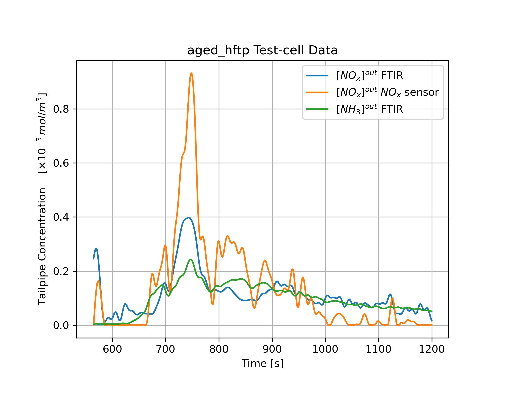
\includegraphics[width=\figWidth]{./figs/2_mdl/fig3_cross_aged_hftp.eps}
        \caption{$\nox$ sensor cross-sensitivity to tailpipe ammonia}
        \label{fig::cross_sensitivity}
\end{figure}
% The FTIR sensor also has a bias that is directional. Similar arguments as above can be made for the validity of the
% bounding condition.
%% === END of: secs/2-subs/2-4-NOx_crosssensitivity.tex ===
%% === END of: secs/2-SatSys_model.tex ===
%% === INLINED from: secs/3-MLE_estimation.tex ===
\section{Maximum Likelihood Estimation of the Model Parameters}

The catalyst switches between saturation mode and normal mode based on states that are not completely controllable
experimentally. The bounding condition on the saturated system's response (\ref{eqn::eta_bound}) can be used for
detecting segments of the data where the catalyst's operation is normal or saturated. As the saturated catalyst's
response forms a tight upper bound to the actual system's response, the parameters of the system will be the solution
to the linear programming problem that minimizes the area under the curve with the lower bound as the response of the
actual system:
\begin{align}
\text{min. } \, \sum \eta_{sat}(k) \quad
\text{s.t } \, \lr{\eta_{sat}(k) \geq \eta(k)} \quad \forall  k \label{eqn::lin_opt_1}
\end{align}
%===
The optimization problem (\ref{eqn::lin_opt_1}) is feasible as $\eta_{sat}$ and $\eta \geq 0$ always. When the $\nox$ sensor
data is used, $\eta(k)$ is replaced with $\eta_y(k)$ as the bounding condition still holds (\ref{eqn::eta_y_bound}).
Rewriting the optimization problem using the regression vector (\ref{eqn::regression}), we have the linear programming
problem for estimating the parameters of the catalyst:
\begin{align}
        \text{minimize} &\qquad \pmb 1^T \lrb{\Phi_{sat} \theta_{sat}}      \label{eqn::lin_prog}\\
        \text{subject to} &\qquad \Phi_{sat} \theta_{sat} \succeq H,  \notag\\
        \text{where } & \qquad
        \Phi_{sat} = \bm{\phi_{sat}(1), \phi_{sat}(2), \hdots, \phi_{sat}(N-1)}^T \notag\\
        &\qquad H = \bm{ \eta(2), \eta(3), \hdots, \eta(N)}^T \notag\\
        & \text{$\pmb 1$ is a column vector of $1's$.} \notag
\end{align}
%===
The above estimate of $\theta_{sat}$ is the \itbf{maximum likelihood estimate (MLE) under a half-normal distribution
\cite{942636} for model structure error}, $\lr{\varepsilon_\eta}$, between the saturated system's response,
$\eta_{sat}(k)$, and the actual response of the catalyst, $\eta(k)$ (Appendix-\ref{sec::mle_derivation}). In the
case of $\nox$-sensor data with cross-sensitivity, the model structure error includes the cross-sensitivity error
$\varepsilon_{\chi}$ and is assumed to be a half-normal random variable.
%===
%% === INLINED from: secs/3-subs/3-1-theta_dist.tex ===
% \subsection{Distribution of the Parameter Estimate}

Using asymptotic properties of MLE (Theorem-7.3 in \cite{kay1993estimation}), with sufficiently large data length
$(N)$, the parameter estimate $\hat \theta_{sat}$ asymptotically follows a normal distribution under some regularity
conditions on the PDF $p(\pmb \varepsilon_n; \theta_{sat})$,
\begin{align}
        \hat \theta_{sat} \sim \mathcal{N} \lr{\theta_{sat},  I^{-1}(\theta_{sat})}
        \label{eqn::theta_dist}
\end{align}
where $I(\theta_{sat})$ is the Fisher information matrix evaluated at the true value of the parameter $(\theta_{sat})$.
The regularity conditions require the existence of derivatives of the log-likelihood function and the Fisher information
being nonzero. Using the log-likelihood function, $L(\theta_{sat})$, for half-normal distribution
(\ref{eqn::log_likelihood}), we have,
\begin{align}
        \lrb{I(\theta_{sat})}_{ij} & = -E \lrb{\frac{\partial^2 L\lr{\theta_{sat}}}{\partial \theta_j
        \partial \theta_i}} = \frac{1}{\sigma^2} {\sum_{k=1}^{N} \frac{\partial \varepsilon_\eta(k)}{\partial \theta_i}\frac{\partial \varepsilon_\eta(k)}{\partial \theta_j}} \notag \\
        I(\theta_{sat})            & = \frac{1}{\sigma^2} \lrb{\Phi_{sat}^T \Phi_{sat}}
        \label{eqn::fisher_information}
\end{align}
%% === END of: secs/3-subs/3-1-theta_dist.tex ===
%% === INLINED from: secs/3-subs/3-2-eta_sat_variance.tex ===
% \subsection{Variance in $\eta_{sat}$ prediction}

$\noindent$ The variance in the $\eta_{sat}$ prediction for the given time-step is obtained by propagating the
uncertainty of parameter estimates (\ref{eqn::theta_dist}). Using (\ref{eqn::regression}), we have,
\begin{align}
        \Var\lrb{\eta_{sat}(k)} &= \phi_{sat}(k)^T I^{-1}(\theta_{sat}) \phi_{sat}(k)
        \label{eqn::eta_sat_var}
\end{align}
%% === END of: secs/3-subs/3-2-eta_sat_variance.tex ===
%% === INLINED from: secs/3-subs/3-3-FTIR_results.tex ===
$\noindent$ The parameter estimates using FTIR measurements from the test-cell experiments are tabulated in
Table~\ref{tab::parm_FTIR}. The parameters show consistency across repeated RMC (Ramped Mode Cycle) and Hot-FTP (Federal
Test Procedure) tests on the same catalyst, which validates the estimation approach. However, the parameters vary
significantly between RMC and Hot-FTP tests. This is predominantly due to the differences in the temperature ranges
experienced by the catalyst during the tests, which affect the Arrhenius temperature dependence of the rate constant
and the concentration of viable voids on the catalyst surface. The temperature range of the data considered during the
RMC tests is between $240^\circ C$ and $360^\circ C$, while for the Hot-FTP tests it is between $200^\circ C$ and $300^\circ C$.
\begin{table}[ht]
        \centering
        \caption{Parameter Estimates using FTIR Data}
        \label{tab::parm_FTIR}
        \begin{tabular}{l c c c c}
                \hline \hline
                Test & $\hat \theta_1 $ & $\hat \theta_2 $ & $\hat \theta_3 $ & $\sigma$\\ \hline \hline
                        DG RMC 1  & -0.63 & 0.55 & 38.74 & 1.14\\
                        DG RMC 2  & -0.82 & 0.69 & 38.61 & 1.08\\
                        DG RMC 3  & -0.80 & 1.12 & 38.78 & 1.10\\
                        Aged RMC  & -1.31 & 1.89 & 36.94 & 1.01\\ \hline
                        DG Hot FTP 1 & -2.14 & -5.80 & 39.53 & 1.35\\
                        DG Hot FTP 2 & -3.45 & -7.99 & 38.05 & 1.30\\
                        DG Hot FTP 3 & -3.37 & -6.42 & 38.88 & 1.33\\
                        Aged Hot FTP & -4.54 & -8.01 & 37.00 & 1.31\\
                \hline\hline
        \end{tabular}
\end{table}
%% === END of: secs/3-subs/3-3-FTIR_results.tex ===
%% === INLINED from: secs/3-subs/3-4-NOx_sensor_results.tex ===
\par The parameter estimates using $\nox$ sensor measurements from the test-cell experiments are tabulated in
Table~\ref{tab::parm_nox}. The parameter estimates are different from those obtained using FTIR measurements
(Table~\ref{tab::parm_FTIR}) due to the cross-sensitivity of the $\nox$ sensor to ammonia. However, the parameters show
consistency across repeated tests on the same catalyst under similar test conditions. The $\nox$ sensor
cross-sensitivity error $\varepsilon_{\chi}(T)$ introduces a bias in the parameter estimates, because the component of
the error that shares the same temperature dependence as the model structure is absorbed into the parameter estimates.
Thus, the linear programming problem estimates the parameters with an added bias term as shown below:
\begin{align}
        \varepsilon_{\chi}(T) & = \phi_{sat}(T(k))^T \theta_{\varepsilon_{\chi}} + \Delta\varepsilon_{\chi}                    \\
        J(\theta_{sat})
                              & = \sum_{k=0}^{N-1} \lr{ \phi^T(k) \lr{\theta_{sat} + \theta_{\varepsilon_{\chi}}} - \eta (k) }
        \label{eqn::nox_cost}
\end{align}
Thus, the estimated parameters using $\nox$ sensor measurements will have a bias dependent on the cross-sensitivity
error characteristics of the sensor used. From the experimental results, it is observed that $\nox$ sensor
cross-sensitivity reduces the difference between the estimates of the aging factor
(Figures~\ref{fig::alpha_sat_ssd} and \ref{fig::alpha_sat_iod}) for aged and degreened catalysts. However, the overall trend
of the change in parameter values remains consistent.
%===
\begin{table}[ht]
        \centering
        \caption{Parameter Estimates using $\nox$ Sensor Data}
        \label{tab::parm_nox}
        \begin{tabular}{l c c c c}
                \hline \hline
                Test         & $\hat \theta_1 $ & $\hat \theta_2 $ & $\hat \theta_3 $ & $\sigma$ \\ \hline \hline
                DG RMC 1     & -0.70            & 0.56             & 38.48            & 1.10     \\
                DG RMC 2     & -1.18            & 0.93             & 38.43            & 1.07     \\
                DG RMC 3     & -0.54            & 0.62             & 38.99            & 1.06     \\
                Aged RMC     & -1.03            & 1.26             & 37.80            & 1.00     \\ \hline
                DG Hot FTP 1 & -2.30            & -6.11            & 37.08            & 1.28     \\
                DG Hot FTP 2 & -2.71            & -6.13            & 36.22            & 1.27     \\
                DG Hot FTP 3 & -3.92            & -6.17            & 35.81            & 1.30     \\
                Aged Hot FTP & -6.42            & -13.06           & 34.73            & 1.34     \\
                \hline\hline
        \end{tabular}
\end{table}
%==
%% === END of: secs/3-subs/3-4-NOx_sensor_results.tex ===
%% === INLINED from: secs/3-subs/3-6-limitations.tex ===
\par Furthermore, the parameter estimation method delineated above has a limitation: the data set must include the response of the catalyst under saturation for a finite duration. If this condition is not met, the algorithm estimates the parameters by treating the maximum concentration of adsorbed ammonia achieved in the data as the concentration corresponding to catalyst saturation (Appendix-\ref{sec::necessary_cond}).
%% === END of: secs/3-subs/3-6-limitations.tex ===
%% === END of: secs/3-MLE_estimation.tex ===
%% === INLINED from: secs/4-catalyst_mode_detection.tex ===
\section{Catalyst Mode Detection}
Under catalyst saturation, the $\nox$ reduction $\lr{\eta_{sat}(k+1)}$ is independent of its previous state
$\lr{\eta_{sat}(k)}$ and initial conditions (\ref{eqn::regression}, \ref{eqn::phi_def}). Rather, it depends entirely on
the inputs from the preceding time step, $\lr{u_1(k), F(k), T(k)}$. Thus, the measured $\nox$ reduction at any given
time step can be classified as either a saturated or an unsaturated response based solely on these prior inputs.
Consequently, by utilizing the estimated parameters, a data point is identified as a saturated-catalyst response if the
prediction error for the corresponding inputs (inlet $\nox$, $u_1$, and mass flow rate $F$) is less than $\epsilon_{sat}$.
\begin{align}
    \abs{\hat \eta_{sat}(k) - \eta(k)} \leq \epsilon_{sat} \implies \text{Catalyst Saturation} \label{eqn::sat_cond}
\end{align}
For the current test-cell and truck data sets, $\epsilon_{sat} = 2.5\times 10^{-3} \, mol/m^{-3}$. This value is chosen
based on the variance of the distribution of the prediction error for the saturated catalyst model.
\begin{figure}[H]
    \centering
%%     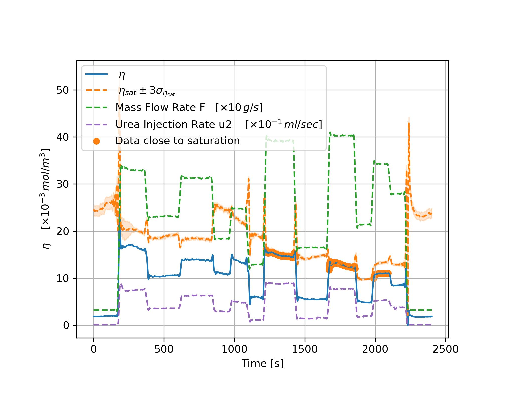
\includegraphics[width=\figWidth]{./figs/4_cat_mode/fig6_SatDetect_dg_rmc_1_FTIR.eps}
    \caption{Catalyst Mode Detection for DG RMC 1 Data}
    \label{fig::cat_mode_det}
\end{figure}
The catalyst mode detection for the degreened (DG) catalyst under RMC 1 test-cell conditions using FTIR measurements is shown in
Figure~\ref{fig::cat_mode_det}. The figure illustrates the operating points for which the prediction error of the
saturated catalyst model satisfies \eqref{eqn::sat_cond}, and are therefore classified as saturated, i.e., close to
maximum $\nox$ reduction. The catalyst is found to be close to saturation when the mass flow rate and the urea dosing
rates are high, consistent with the physical understanding of the catalyst operation. Furthermore, the flow rate can
introduce a virtual ceiling on the maximum achievable $\nox$ reduction due to reduced residence time in the catalyst,
which would be indistinguishable from saturated-catalyst behavior, since the $\nox$ reduction would be independent of
urea dosing.

A fraction of the data from the test-cell experiments under RMC and Hot-FTP test conditions for both degreened and aged
catalysts is found to be in saturated mode. The number of data points close to catalyst saturation $\lr{N_{sat}}$ and
the total number of samples ($N$) for different test conditions are listed in Tables~\ref{tab::sat_data_perc_ssd} and
\ref{tab::sat_data_perc_iod}. The total number of data points, $N$, is the total length of the temporally contiguous
segment of the test cell data that is within the chosen temperature operating range for the tests. The operating range
for RMC test is between $250^\circ C$ and $350^\circ C$, and for Hot-FTP test is between $200^\circ C$ and $300^\circ
    C$.
%==============================================================
\begin{table}[ht]
    \centering
    \caption{Data Points Close to Catalyst Saturation in Test-Cell FTIR Data}
    \label{tab::sat_data_perc_ssd}
    \begin{tabular}{l r r r}
        \hline \hline
        Test         & $N$  & $N_{sat}$ & $\% \lr{ \sfrac{N_{sat}}{N} }$ \\\hline \hline
        DG RMC 1     & 2402 & 490       & 20.4                           \\
        DG RMC 2     & 2402 & 493       & 20.5                           \\
        DG RMC 3     & 2402 & 491       & 20.4                           \\
        Aged RMC     & 2402 & 515       & 21.4                           \\ \hline
        DG Hot FTP 1 & 634  & 186       & 29.3                           \\
        DG Hot FTP 2 & 634  & 181       & 28.5                           \\
        DG Hot FTP 3 & 638  & 180       & 28.2                           \\
        Aged Hot FTP & 636  & 198       & 31.1                           \\
        \hline\hline
    \end{tabular}
\end{table}
\begin{table}[ht]
    \centering
    \caption{Data Points Close to Catalyst Saturation in Test-Cell $\nox$ Sensor Data}
    \label{tab::sat_data_perc_iod}
    \begin{tabular}{l r r r}
        \hline \hline
        Test         & $N$  & $N_{sat}$ & $\% \lr{ \sfrac{N_{sat}}{N} }$ \\\hline \hline
        DG RMC 1     & 2402 & 492       & 20.5                           \\
        DG RMC 2     & 2402 & 494       & 20.6                           \\
        DG RMC 3     & 2402 & 493       & 20.5                           \\
        Aged RMC     & 2402 & 515       & 21.4                           \\ \hline
        DG Hot FTP 1 & 634  & 194       & 30.6                           \\
        DG Hot FTP 2 & 634  & 191       & 30.1                           \\
        DG Hot FTP 3 & 638  & 198       & 31.0                           \\
        Aged Hot FTP & 636  & 220       & 34.6                           \\
        \hline\hline
    \end{tabular}
\end{table}
Note that the higher number of data points classified as close to catalyst saturation in RMC test conditions, compared
to Hot-FTP, results in better parameter estimates and performance of the aging detection test statistic in this case
(Table~\ref{tab::Tw_tst}).
%% === END of: secs/4-catalyst_mode_detection.tex ===
%% === INLINED from: secs/5-catalyst_aging.tex ===
\section{Model Parameters Capture Catalyst Aging}
The parameters of the saturated system are a function of the rate constant for the SCR reaction and the maximum surface
concentration of viable voids on the catalyst. The adsorption site concentration is hypothesized to change with catalyst aging, allowing the estimated parameters to capture this degradation. This is demonstrated using the test-cell
experiments on a new (degreened) and hydrothermally aged catalyst with the same capacity. The predicted $\nox$
reduction for an aged catalyst is found to be statistically lower than the predicted $\nox$ reduction in a degreened
catalyst (Figure~\ref{fig::aging_diff}). The dashed line in Figure~\ref{fig::aging_diff} corresponds to the actual response of the reference system, whose inputs are used to predict the saturated system's response using parameter estimates from the degreened and aged catalyst data under RMC test conditions. Thus, in accordance with the bounding condition (\ref{eqn::eta_bound}), the actual response is always less than the predicted saturated system's response.
\begin{figure}[ht]
        \centering
%%         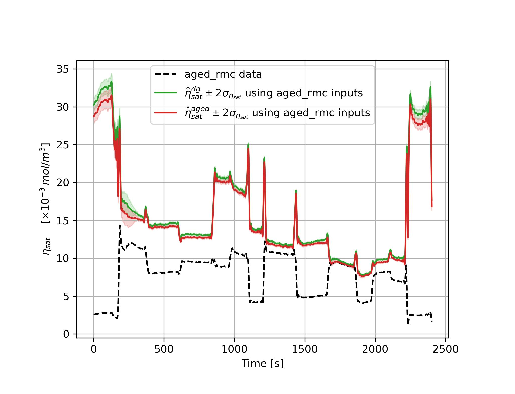
\includegraphics[width=\figWidth]{./figs/5_aging/fig7_AgingDiff.eps}
        \caption{Predicted $\eta_{sat}$ for Aged and Degreened Catalyst}
        \label{fig::aging_diff}
\end{figure}
%===
When the $\eta_{sat}$ response is normalized with respect to the inlet $\nox$ concentration and flow rate, we obtain
a quantity that is only a function of temperature and represents the product of the rate constant and maximum surface
coverage. From (\ref{eqn::regression}),
\begin{align}
        \alpha_{sat} &= \frac{F(k)}{u_1(k)} \eta_{sat}(k) = \tau_0 k_{scr}\Gamma = \phi_T^T(k)\theta_{sat}\\
        \text{where} \quad \phi_T^T(k) &= \bm{2\lr{\frac{T-T_0}{T_r}}^2-1 & \frac{T-T_0}{T_r} & 1}
\end{align}
%===
This quantity, $\alpha_{sat}$, can be estimated and changes with catalyst aging, based on the hypothesis that aging
affects the adsorption site concentration. The change in $\alpha_{sat}$ with aging is demonstrated using the test-cell
experiments (Figures~\ref{fig::alpha_sat_ssd} and \ref{fig::alpha_sat_iod}). The variance is estimated by propagating
the variance of the $\eta_{sat}$ estimate (\ref{eqn::eta_sat_var}). As expected from the cost function for parameter
estimation under $\nox$ sensor cross-sensitivity (\ref{eqn::nox_cost}), the parameter estimates have a bias that reduces
the difference between the estimates for the degreened and aged catalysts. However, the overall trend of change in
parameter values with aging remains consistent across both FTIR and $\nox$ sensor measurements.
\begin{figure}[ht]
        \centering
%%         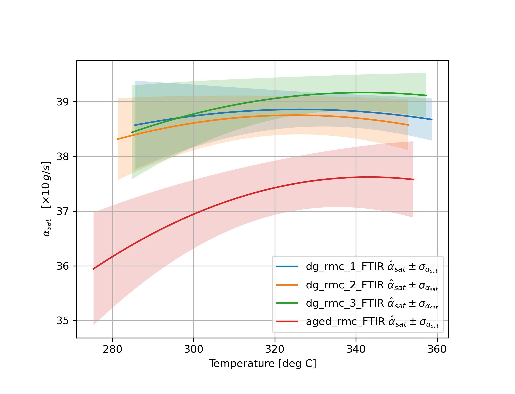
\includegraphics[width=\figWidth]{./figs/5_aging/fig8_aging_factor_ssd.eps}
        \caption{$\hat \alpha_{sat}$ from RMC FTIR Data}
        \label{fig::alpha_sat_ssd}
\end{figure}
\begin{figure}[ht]
        \centering
%%         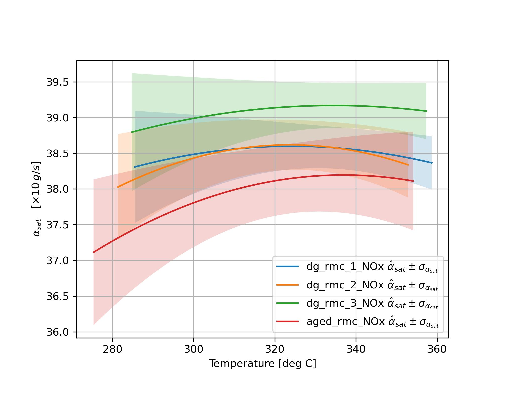
\includegraphics[width=\figWidth]{./figs/5_aging/fig9_aging_factor_iod.eps}
        \caption{$\hat \alpha_{sat}$ from RMC $\nox$ Sensor Data}
        \label{fig::alpha_sat_iod}
\end{figure}
%===
\par Thus, $\theta_{sat}$ captures the aging of the catalyst. Hence, the catalyst aging detection problem can be posed
as a hypothesis-testing problem, with the null hypothesis $\lr{\mathcal{H}_0}$ corresponding to a degreened catalyst and
the alternative hypothesis $\lr{\mathcal{H}_1}$ corresponding to an aged catalyst. Since the distribution of the error is
assumed to be known (half-normal) for both hypotheses and differs by the unknown parameter $\theta_{sat}$, which can be
estimated, the following Wald test \cite{wald1943tests} is proposed to check whether the parameter estimates for a given
data set correspond to an aged catalyst or a known degreened catalyst.
Decide $\mathcal{H}_1$ if,
\begin{align}
        T_w  &= \lr{\hat \theta_{sat} - \theta_{sat}^{dg}}^T I\lr{\hat \theta_{sat}} \lr{\hat \theta_{sat} - \theta_{sat}^{dg}} > \beta \label{eqn::wald_test}
\end{align}
where $\theta_{sat}^{dg}$ is the parameter estimate for the degreened catalyst under the same input conditions,
including temperature, flow rate, and urea-dosing rate ranges. The threshold $\beta$ is chosen based on the experimental
results. For the RMC and FTP data sets, the values of the test statistic are tabulated in Table~\ref{tab::Tw_tst}.
% Table of test-statistic
\begin{table}[ht]
        \centering
        \caption{Wald Test Results on the Test-Cell Data}
        \label{tab::Tw_tst}
        \begin{tabular}{l c c}
        \hline \hline
        Test & $T_w$ from FTIR & $T_w$ from $\nox$ sensor \\\hline \hline
        DG RMC 1      & 0.26 & 5.54\\
        DG RMC 2      & 0.00 & 0.00\\
        DG RMC 3      & 6.71 & 5.46\\
        Aged RMC      & 47.16 & 17.68\\
        \hline
        DG Hot FTP 1  & 0.49 & 0.81\\
        DG Hot FTP 2  & 3.26 & 1.98\\
        DG Hot FTP 3  & 0.00 & 0.00\\
        Aged Hot FTP  & 4.84 & 11.44\\
        \hline \hline
        \end{tabular}
\end{table}
The distribution of the test statistic under aging (non-central $\chi^2$, asymptotically) is different for the RMC and FTP
test conditions due to differences in the ranges of inputs (temperature, flow rate, and urea-dosing rate) experienced
by the catalyst during the tests. Based on the results, a reasonably discerning threshold that maximizes the probability of detection for both Hot-FTP and RMC test conditions is found to be
\begin{align}
        \beta_{hFTP} &= 4.00, \qquad \beta_{RMC} = 10.00
\end{align}
Further investigation with more data is needed to determine the probabilities of detection and false alarm for these
thresholds. The proposed Wald test detects the aged catalyst for both FTIR and $\nox$ sensor measurements under both
test conditions.
%% === END of: secs/5-catalyst_aging.tex ===
%% === INLINED from: secs/6-trucks.tex ===
\section{Aging Detection from Truck Data}
%===
The performance of the proposed aging detector is also demonstrated using the $\nox$ sensor data from four long-haul
trucks. The road data were collected from trucks operating in the United States for two days separated by a few years
(Table~\ref{tab::truck_data_summary}) during which the catalyst had aged based on existing performance measures. The
data has measurements of $\nox$ sensors before and after the catalyst, as well as other required variables
including flow rate, temperature and urea injection rate. The data preprocessing includes,
\begin{inparaenum}
        \item removing the rows with missing values,
        \item removing the rows whose operating temperature range is beyond the range of $200-300 \,^\circ C$,
        \item interpolating the missing data if the data gaps are smaller than a minute, and finally,
        \item smoothing the data using a non-causal Chebyshev filter.
\end{inparaenum}
The preprocessed data is then partitioned into drive segments with no breaks, which correspond to a continuous driving
period from engine start to engine stop.
%===
% Truck Mapping
% Truck A - AD Transport (adt)
% Truck B - Mesilla Valley (mes)
% Truck C - Werner (wer)
% Truck D - Transwest (trw)
% =====
\begin{table}[ht]
        \centering
        \caption{Truck Data Set Years and Mileage Difference}
        \label{tab::truck_data_summary}
        \begin{tabular}{c c c c}
                \hline \hline
                Truck   & Earlier Data & Latter Data & Mileage            \\
                        & Year         & Year        & Difference         \\ \hline \hline
                Truck A & $2015$       & $2017$      & $2.8 \times 10^5$  \\
                Truck B & $2015$       & $2018$      & $11.9 \times 10^5$ \\
                Truck C & $2015$       & $2017$      & $5.9 \times 10^5$  \\
                Truck D & $2015$       & $2016$      & $6.6 \times 10^5$  \\
                \hline \hline
        \end{tabular}
\end{table}
%===
Unlike the test-cell data where the engine drive-cycles are repeatable and produce a significant fraction of samples where the catalyst is close to saturation, the truck data drive segments constitute varied driving conditions with fewer samples $\lrf{\leq 10\%}$ that are close to catalyst saturation. A necessary condition for the proposed parameter estimation and aging detection framework is that the data has a sufficiently large number of samples close to catalyst saturation such that the asymptotic properties of the MLE and the test statistic hold (\ref{eqn::Ns_min}). Hence, the drive segment data are further pruned to only include segments with at least $150$ samples ($120$ in the case of Truck C) close to catalyst saturation.
\begin{align}
        N_{sat}       & \geq N_{sat}^{min} \label{eqn::Ns_min} \\
        \beta_{truck} & = 250 \label{eqn::beta_truck}
\end{align}
The threshold of the Wald test statistic (\ref{eqn::beta_truck}) for aging detection in trucks is chosen such that it
maximizes the probability of detection while minimizing the probability of false alarm and missed detection for the
given limited truck data. The value of the test statistic for the drive segments for each truck is tabulated in
Tables~\ref{tab::adt_aging_res}, \ref{tab::mes_aging_res}, \ref{tab::wer_aging_res} and \ref{tab::trw_aging_res}. A
summary of the aging detection results is tabulated in Table~\ref{tab::truck_aging_summary}. The detector performs
reasonably well on three of the four trucks with high probability of detection and low false alarm and missed detection
rates. Truck A has relatively lower mileage difference between the earlier and latter data years which may explain the
lower detection performance. The performance is limited by the amount of data available with sufficient samples close to
catalyst saturation. Further, the lack of ground truth on the actual individual catalyst's aging levels limits the
ability to quantify the performance of the detector.
%===
\begin{table}[ht]
        \centering
        \caption{Summary of Aging Detection Results on Truck Data}
        \label{tab::truck_aging_summary}
        \begin{tabular}{c c c c c}
                \hline \hline
                Truck   & Total Drive & Detection & False & Missed    \\
                        & Segments    &           & Alarm & Detection \\\hline \hline
                Truck A & 8           & 4         & 0     & 4         \\
                Truck B & 11          & 9         & 1     & 1         \\
                Truck C & 9           & 7         & 1     & 1         \\
                Truck D & 8           & 6         & 2     & 0         \\
                \hline \hline
        \end{tabular}
\end{table}
%===

The threshold $\beta_{truck} = 250$ is significantly larger than the test-cell thresholds ($\beta_{RMC} = 10$,
$\beta_{hFTP} = 4$) because the limited sample size causes $T_w$ to diverge from its asymptotic $\chi^2_\nu$
distribution under $\mathcal{H}_0$. The convergence of the MLE to normality depends on the number of saturated-mode
samples \cite{kay1993estimation}, and truck data has considerably fewer such samples ($N_{sat} \approx 120$-$150$)
compared to test-cell experiments ($N_{sat} \approx 200$-$500$), resulting in heavier tails in the null distribution of
$T_w$. This effect is compounded by the less reliable estimation of the error variance under road conditions and the
unaccounted variance of the reference parameter $\theta_{sat}^{dg}$, which is itself estimated from limited data. Both
factors inflate $T_w$ under $\mathcal{H}_0$, necessitating a higher threshold to maintain an acceptable false-alarm
rate.

With a larger data set and known degreened paramters, the thresholds can be determined using statistically-optimal
selection criteria such as Neyman-Pearson \cite{kay1998detection} or minimum Bayes cost on the receiver operating
characteristic (ROC) curve \cite{PoorDetection}. This would require multiple truck runs under known catalyst conditions
to characterize the null distribution, and runs at known aging levels to estimate the non-centrality parameter under
$\mathcal{H}_1$. Nevertheless, the results demonstrate that the proposed saturated-catalyst model (\ref{eqn::nox_mdl})
coupled with the constrained parameter estimation method (\ref{eqn::lin_prog}) and the statistical detector
(\ref{eqn::wald_test}) enables a statistically-grounded aging detection framework that performs reasonably well on both
test-cell and truck data under sensor sampling limitations and cross-sensitivity.

%=== Practical OBD considerations ===
For on-vehicle implementation, the detector's performance depends on whether the driving profile produces sufficient
data close to catalyst saturation within a given driving window. Conditions that combine moderate-to-high exhaust mass
flow rates with elevated urea dosing, such as sustained highway cruising, high-load acceleration, or uphill driving
within the detector's operational temperature range ($200$--$300\,^\circ C$ in the present case, which can be adjusted),
are most likely to trigger saturation. The extent of catalyst utilization can be assessed in real time by monitoring
readily-available signals such as urea dosing rate, engine rpm, and the estimate of $\nox$ reduction from sensors. When
these indicate sustained low $\text{NO}_x$ reduction and low urea dosing which leaves the catalyst unsaturated, the
system can determine apriori that the accumulated data are unsuitable for aging detection and defer its decision rather
than executing the hypothesis test on insufficient data. The detector therefore avoids producing false alarms under
non-catalyst-saturating driving conditions, as the Wald test~(\ref{eqn::wald_test}) is simply not invoked. A consequence
of this design is that the monitor's in-use performance ratio (IUPMR) is governed by the frequency of saturating driving
conditions, since the diagnostic can only complete when the necessary condition~(\ref{eqn::Ns_min}) is met.


%% === END of: secs/6-trucks.tex ===
%% === INLINED from: secs/7-conclusion.tex ===
\section{Conclusion}
%===
The dynamics of $\nox$ reduction in diesel engine SCR systems under catalyst saturation were used to develop an aging
detector based on the hypothesis that the model parameters associated with catalyst storage capacity change as the
catalyst ages. A dynamic model for $\nox$ reduction under saturation was formulated from molar conservation while
explicitly accounting for the interplay between the residence time of the reacting flow and the sampling time of the
sensors. A maximum-likelihood parameter estimation algorithm was proposed using the bounding condition between the
actual system response and the response under catalyst saturation. The algorithm was validated using experimental
test-cell data under RMC and Hot-FTP conditions. The $\nox$-sensor's ammonia cross-sensitivity, in the absence of a
dedicated ammonia sensor, was shown to introduce a bias in the parameter estimates, reducing the separation between the
estimates for degreened and aged catalysts. A catalyst mode detection method was utilized to identify data segments
operating near saturation. A hypothesis-testing framework based on the Wald test was then developed for catalyst aging
detection using the estimated parameters. The detector's performance was demonstrated using test-cell data at different
aging levels and real-world data from four long-haul trucks. The results indicate that the proposed framework can
reliably identify catalyst aging even in the presence of sensor cross-sensitivity and varying operating conditions,
provided that the data include a sufficient number of samples near the saturation regime, which forms a necessary
condition for aging detection.
%% === END of: secs/7-conclusion.tex ===

%=======================================================================================================================
\section*{Acknowledgment}
Authors acknowledge the support and feedback from David Schmidt, Larry Bruner, Adam Kidd and Tom Nelson of Cummins, Inc.
%=======================================================================================================================
\section*{Funding Data}
Authors acknowledge the funding and test-cell, truck and simulation data of Diesel Engine Aftertreatment Systems from Cummins, Inc.
%=======================================================================================================================
%% === INLINED from: secs/0-symb_list.tex ===
%\EntryHeading{Greek Letters}

\begin{nomenclature}
    \EntryHeading{Symbols}
    \entry{$\lrf{\bullet}$}{Number of moles of $\bullet$. $(moles)$}
    \entry{$\lrb{\bullet}$}{Concentration of $\bullet$. $(mol/m^3)$}
    \entry{$A_{scr}$}{Pre-exponential factor of SCR reaction}
    \entry{$E_{scr}$}{Activation Energy of SCR reaction}
    \entry{$F$}{Mass flow rate of the exhaust gases $(g/s)$}
    \entry{$I(\theta)$}{Fisher Information Matrix}
    \entry{$k_i$}{Coefficients of polynomial temperature model for $k_{scr}$}
    \entry{$N_{sat}$}{Number of data points close to catalyst saturation}
    \entry{$N$}{Total number of data points}
    \entry{$N_{sat}^{min}$}{Minimum number of data points close to catalyst saturation for reliable parameter estimation}
    \entry{$r_i$}{Coefficients of polynomial temperature model for $\Gamma$}
    \entry{$R$}{Universal gas constant}
    \entry{$S_1, S_2$}{Coefficients of the temperature model for $\Gamma$, $S_1, S_2 \geq 0$}
    \entry{$T$}{Temperature}
    \entry{$T_w$}{Wald test statistic for catalyst aging detection}
    \entry{$u_1$}{Engine-out (SCR-in) $\nox$ concentration}
    \entry{$V_{scr}$}{Volume of the catalyst chamber}
    \entry{$x_1$}{Tailpipe (SCR-out) $\nox$ concentration}
    \entry{$y_1$}{Tailpipe (SCR-out) $\nox$ sensor measurement}
    \entry{$\alpha_{sat}$}{Flow and inlet $\nox$ normalized $\nox$ reduction under catalyst saturation}
    \entry{$\beta$}{Threshold for Wald test statistic for catalyst aging detection}
    \entry{$\gamma(k)$}{Average surface concentration of adsorbed ammonia in the sample [k] to [k+1]}
    \entry{$\Gamma $}{Surface concentration of the total storage capacity for the catalyst $(mol/m^2)$}
    \entry{$\varepsilon_\chi$}{Error in $\nox$ due to ammonia cross-sensitivity}
    \entry{$\varepsilon_\eta$}{Model structure error between saturated catalyst model and actual system}
    \entry{$\eta_{sat}$}{$\nox$ reduction per time-step under catalyst saturation}
    \entry{$\phi_{sat}(T)$}{Regression vector for saturated catalyst model}
    \entry{$\rho$}{Density of the exhaust gases}
    \entry{$\sigma_{\eta}$}{Standard deviation in $\nox$ }
    \entry{$\sigma$}{Scale parameter for half-normal distribution}
    \entry{$\theta_{sat}$}{Parameter vector for saturated catalyst model}
    \entry{$\theta_{sat}^{dg}$}{Parameter estimates for degreened catalyst}
    \entry{$\chi$}{Cross-sensitivity factor}
    %===

    \EntryHeading{Abbreviations}
    \entry{ASC}{Ammonia Slip Catalyst}
    \entry{CSTR}{Continuously Stirred Tank Reactor}
    \entry{DG}{Degreened}
    \entry{FTP}{Federal Test Procedure}
    \entry{IUMPR}{In-Use Performance Ratio}
    \entry{MLE}{Maximum Likelihood Estimate}
    \entry{PDF}{Probability Density Function}
    \entry{PFR}{Plug Flow Reactor}
    \entry{RMC}{Ramped Mode Cycle}
    \entry{ROC}{Receiver Operating Characteristic}
    \entry{SCR}{Selective Catalytic Reduction}
\end{nomenclature}
%% === END of: secs/0-symb_list.tex ===
%=======================================================================================================================
\appendix   %%% starting appendices
%% === INLINED from: secs/n-appendix.tex ===
%====
% \section{Limitations of Polynomial Models for Temperature Dependence}

The regression model (\ref{eqn::regression}) interpolates the exponential temperature dependence of the term
$k_{scr}\Gamma$ using a quadratic. This approximation introduces an error but results in a linear in parameters model
with unique solution under least-squares for interpolation. The model identified from the data has a strong dependence
on the temperature characteristics of the experimental data. Fitting a quadratic temperature model for the response of a
nonlinear function of temperature in least-squares sense involves inverting the following matrix, $\Lambda$, which is
only a function of the temperature sampling and multiplying it to a vector that is a function of the output of nonlinear function at the temperature samples.
\begin{align}
        \Lambda = \frac{1}{N}\bm{\sum T_i^4 & \sum T_i^3 & \sum T_i^2\\
                                 \sum T_i^3 & \sum T_i^2 & \sum T_i^1\\
                                 \sum T_i^2 & \sum T_i^1 & N\\  }  \qquad i \in & \lrf{1, 2, \hdots, N}
\end{align}
Thus, one way to ensure that the parameter estimates are comparable across data sets is to require that the sufficient statistics, which are solely functions of temperature, remain the same (or approximately so).
\begin{align}
        %\min{\lr{T_i}},  \max{\lr{T_i}} &       \label{eqn::T_suff_1}\\
        \frac{\sum T_i}{N}, \frac{\sum{T_i^2}}{N}, \frac{\sum{T_i^3}}{N}, \text{ and } \frac{\sum{T_i^4}}{N} \qquad i \in & \lrf{1, 2, \hdots, N}       \label{eqn::T_suff_2}
\end{align}
Although these conditions are stringent, they can be satisfied through a judicious selection of data segments. Given
that the operating temperature range of the catalyst is finite, the minimum and maximum temperatures can be defined
accordingly. Subsequently, data segments may be included or excluded based on whether the corresponding sufficient
statistics satisfy the prescribed criteria. Furthermore, if the prediction error becomes significantly large, the model can be partitioned to enable switching between distinct temperature zones.

%===
%% === INLINED from: secs/3-subs/3-0-Apx-MLE_derivation.tex ===
\section{Maximum Likelihood Estimate Derivation \label{sec::mle_derivation}}
Consider,
\begin{align}
        \varepsilon_\eta(k) & = \eta_{sat}(k) - \eta\lr{k}  \quad
        \implies            & \varepsilon_\eta(k) = \lr{\phi_{sat}^T \theta_{sat} - \eta \lr{k}} \label{eqn::eta_regression}
\end{align}
based on the measurement sensors. Assuming $\varepsilon_\eta$ follows half-normal distribution \cite{byers2014half} with scale-parameter, $\sigma$,
\begin{align}
        \varepsilon_\eta & \backsim \text{Half-Normal}(\sigma);\quad
        p(\varepsilon_\eta;\sigma) = \begin{cases} \frac{\sqrt{2}}{\sigma \sqrt{\pi}} e^{- \frac{\varepsilon_\eta^2}{2 \sigma^2}} & \varepsilon_\eta \geq  0 \\
              0                                                                              & \varepsilon_{\eta} < 0
                                     \end{cases}
        \label{eqn::exp_pdf}
\end{align}
we have the likelihood and log-likelihood functions given the data and parameter estimate $\theta_{sat}$ and $\sigma$:
\begin{align}
        l\lr{\theta_{sat}} & =p(\pmb \varepsilon_{\eta};\theta_{sat}, \sigma) = \prod_{k=1}^N  \frac{\sqrt{2}}{\sigma \sqrt{\pi}} e^{- \frac{\varepsilon_\eta^2}{2 \sigma^2}} \quad \varepsilon_\eta(k) \geq  0
        \label{eqn::likelihood}                                                                                                                                                                                 \\
        L\lr{\theta_{sat}} & =\ln \lr{l(\theta_{sat})} = \frac{N}{2} \ln \frac{2}{\sigma^2 \pi} - \frac{1}{2 \sigma^2} {\sum_{k=1}^N \varepsilon_\eta^2}
        \quad \varepsilon_\eta(k) \geq  0
        \label{eqn::log_likelihood}
\end{align}
where $N$ is the total sample size. The maximum likelihood estimate for $\theta_{sat}$ would be:
\begin{align}
        \hat \theta_{sat}
         & = \argmax_{\theta_{sat}} \lrf{ \frac{N}{2} \ln \frac{2}{\sigma^2 \pi} - \frac{1}{2 \sigma^2} {\sum_{k=1}^N \varepsilon_\eta^2} } \quad \varepsilon_\eta(k) \geq  0 \notag \\
         & = \argmin_{\theta_{sat}} \lr{\sum_{k=1}^N \varepsilon_\eta^2} \quad \varepsilon_\eta(k) \geq  0 \notag                                                                    \\
         & = \argmin_{\theta_{sat}} \lr{\sum_{k=1}^N \lr{\phi_{sat}(k)^T \theta_{sat} - \eta(k)}^2} \notag                                                                           \\
         & \quad  s.t \quad \phi_{sat}(k)^T \theta_{sat} \geq \eta(k) \quad \forall \: k \in {1,2, \hdots, N}
        \label{eqn::quad_prog}
\end{align}
The quadratic program with a positivity constraint can be relaxed to a linear program as follows. By norm equivalence,
the $l_2-$norm in (\ref{eqn::quad_prog}) is replaced with the $l_1$-norm, and the nonnegativity constraint renders the
absolute value redundant, yielding the linear programming formulation in (\ref{eqn::lin_prog_final}).
\begin{align}
        \hat \theta_{sat}
         & = \argmin_{\theta_{sat}} \lr{\sum_{k=1}^N \lr{\phi_{sat}(k)^T \theta_{sat}}} \notag                \\
         & \quad  s.t \quad \phi_{sat}(k)^T \theta_{sat} \geq \eta(k) \quad \forall \: k \in {1,2, \hdots, N}
        \label{eqn::lin_prog_final}
\end{align}
%% === END of: secs/3-subs/3-0-Apx-MLE_derivation.tex ===
%% === INLINED from: secs/3-subs/3-1-Apx-necessary_condition.tex ===
\section{Limitation: Parameter Estimation Assumes Catalyst Saturation \label{sec::necessary_cond}}

The catalyst mode detection algorithm presented fails when the catalyst is not saturated for a
significant length of time in the data. If the data set does not have any regions of saturation, the approach fits a
saturated model as if the maximum achieved catalyst ammonia storage, $(\max\lr{\sigma(k)})$, is the storage capacity of
the catalyst $(\Gamma)$. This is demonstrated using data from high-fidelity simulation model (AVL Cruise
\cite{AVLCruise}) tuned to RMC (Ramped Mode Cycle) test on a test-cell. The RMC test is then simulated with $\pm 20\%$
change in the gain of the urea-dosing controller to change the duration for which the catalyst remains saturated.
\begin{figure}[ht]
        \centering
%%         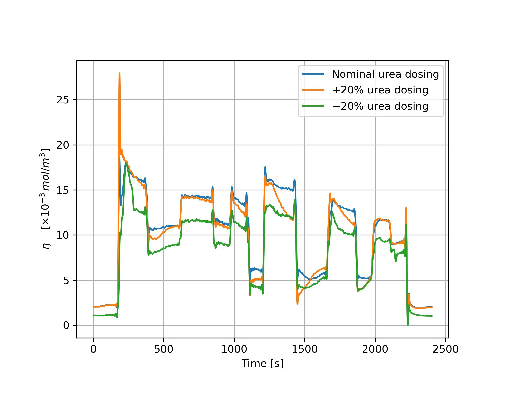
\includegraphics[width=\figWidth]{./figs/3_parm_ID/apx_necessary/fig4_eta_sim.eps}
        \caption{RMC $\eta$ simulation with $\pm 20\%$ Urea Dosing}
        \label{fig::necessary_cond_sim}
\end{figure}
\begin{figure}[ht]
        \centering
%%         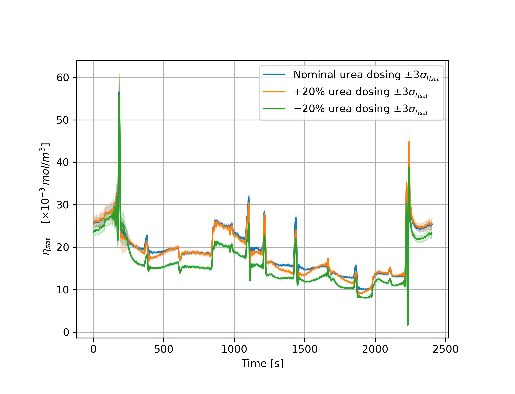
\includegraphics[width=\figWidth]{./figs/3_parm_ID/apx_necessary/fig5_eta_sat.eps}
        \caption{RMC $\eta_{sat}$ prediction with $\pm 20\%$ Urea Dosing}
        \label{fig::necessary_cond_sat}
\end{figure}
Figure-\ref{fig::necessary_cond_sim} shows the actual $\nox$ reduction $(\eta)$ from the simulation under the three dosing conditions, while Figure-\ref{fig::necessary_cond_sat} shows the corresponding predicted saturated-model response $(\eta_{sat})$ using parameters estimated from each case.
Figure-\ref{fig::necessary_cond_sim} shows no increase in $\nox$ reduction when urea dosing is increased by $20\%$,
which indicates that maximum $\nox$ reduction is already reached at nominal urea dosing. This could be because the
catalyst is saturated or because the inlet $\nox$ concentration is sufficiently low. Conversely, a $20\%$ decrease in
urea dosing decreases $\nox$ reduction. When the $-20\%$ urea-dosing data are used to estimate saturated-model
parameters, the model predicts a substantially lower $\nox$ reduction under saturation than for the nominal and $+20\%$
dosing cases (Figure-\ref{fig::necessary_cond_sat}), the latter two giving essentially identical results. Thus, for the nominal and $+20\%$ dosing cases, the catalyst is indeed saturated, and the parameter estimates show the same. However, for the $-20\%$ dosing case, the catalyst is not saturated in the data; instead, the parameters fit the maximum surface coverage achieved $\lrf{\theta_{max} = \sfrac{\gamma_{max}}{\Gamma}}$ in the data, i.e.,
\begin{align}
        \eta_{sat}(k+1) & = \frac{u_1(k)}{F(k)} \tau_0 \; k_{scr} \Gamma \theta_{max} = \phi_{sat} \theta_{sat}
\end{align}

It is assumed that under ordinary drive conditions, the catalyst will reach saturation for a significant length of time, making the proposed parameter estimation approach applicable. In practice, the extent of catalyst utilization over a given data window can be assessed by monitoring readily available signals such as urea dosing rate, engine rpm, and the estimate of $\nox$ reduction from sensors. to verify whether this assumption holds before executing the detector.
%% === END of: secs/3-subs/3-1-Apx-necessary_condition.tex ===
%% === INLINED from: secs/6-subs/6-0-Apx_Truck.tex ===
\section{Aging Detector Results on Truck Data Drive Segments}
The Wald test statistics, along with the counts and percentages of near-saturation samples, are computed for all qualifying drive segments. Results for Trucks A, B, C and D are provided in Tables~\ref{tab::adt_aging_res}, \ref{tab::mes_aging_res}, \ref{tab::wer_aging_res} and \ref{tab::trw_aging_res}, respectively. In each table, entries above and below the horizontal rule correspond to the earlier and latter data years (Table~\ref{tab::truck_data_summary}). The data demonstrate a strong correlation between successful aging detection and the number of near-saturation samples available in a given segment.
%===
% Truck Mapping
% Truck A - AD Transport (adt)
% Truck B - Mesilla Valley (mes)
% Truck C - Werner (wer)
% Truck D - Transwest (trw)
% =====
\begin{table}[H]
        \centering
        \caption{Aging Detection Results for Truck A}
        \label{tab::adt_aging_res}
        \begin{tabular}{l r r r}
                \hline \hline
                Drive Segment & $T_w$  & $N_{sat}$ & $\% \lr{ \sfrac{N_{sat}}{N} }$ \\ \hline \hline
                A$\_15\_0$    & 0.00   & 797       & 6.70                           \\
                A$\_15\_1$    & 28.95  & 305       & 2.75                           \\
                A$\_15\_2$    & 58.50  & 276       & 5.93                           \\
                A$\_15\_3$    & 89.56  & 271       & 12.77                          \\ \hline
                A$\_17\_0$    & 65.59  & 414       & 2.97                           \\
                A$\_17\_1$    & 127.79 & 614       & 6.76                           \\
                A$\_17\_2$    & 12.13  & 330       & 8.44                           \\
                A$\_17\_3$    & 61.76  & 336       & 9.73                           \\
                \hline \hline
        \end{tabular}
\end{table}
%===
\begin{table}[H]
        \centering
        \caption{Aging Detection Results for Truck B}
        \label{tab::mes_aging_res}
        \begin{tabular}{l r r r}
                \hline \hline
                Drive Segment & $T_w$   & $N_{sat}$ & $\% \lr{ \sfrac{N_{sat}}{N} }$ \\ \hline \hline
                B$\_15\_0$    & 672.43  & 167       & 1.26                           \\
                B$\_15\_1$    & 106.66  & 189       & 1.81                           \\
                B$\_15\_3$    & 237.79  & 159       & 2.95                           \\
                B$\_15\_4$    & 0.00    & 226       & 6.03                           \\
                B$\_15\_6$    & 84.73   & 179       & 5.75                           \\ \hline
                B$\_18\_0$    & 543.55  & 231       & 2.10                           \\
                B$\_18\_1$    & 1050.24 & 308       & 3.00                           \\
                B$\_18\_4$    & 22.48   & 195       & 6.14                           \\
                B$\_18\_6$    & 7150.19 & 378       & 12.73                          \\
                B$\_18\_7$    & 760.89  & 224       & 8.14                           \\
                B$\_18\_8$    & 342.67  & 246       & 9.04                           \\
                \hline \hline
        \end{tabular}
\end{table}
% ===
\begin{table}[H]
        \centering
        \caption{Aging Detection Results for Truck C}
        \label{tab::wer_aging_res}
        \begin{tabular}{l r r r}
                \hline \hline
                Drive Segment & $T_w$   & $N_{sat}$ & $\% \lr{ \sfrac{N_{sat}}{N} }$ \\ \hline \hline
                C$\_15\_1$    & 0.000   & 186       & 1.30                           \\
                C$\_15\_4$    & 113.86  & 143       & 3.84                           \\
                C$\_15\_5$    & 4340.08 & 124       & 4.16                           \\ \hline
                C$\_17\_0$    & 700.88  & 186       & 1.24                           \\
                C$\_17\_2$    & 3993.85 & 446       & 7.23                           \\
                C$\_17\_3$    & 1693.49 & 199       & 4.00                           \\
                C$\_17\_4$    & 186.64  & 120       & 2.81                           \\
                C$\_17\_7$    & 1878.52 & 129       & 4.73                           \\
                C$\_17\_9$    & 7500.10 & 218       & 11.63                          \\
                \hline \hline
        \end{tabular}
\end{table}
%=====
\begin{table}[H]
        \centering
        \caption{Aging Detection Results for Truck D}
        \label{tab::trw_aging_res}
        \begin{tabular}{l r r r}
                \hline \hline
                Drive Segment & $T_w$   & $N_{sat}$ & $\% \lr{ \sfrac{N_{sat}}{N} }$ \\ \hline \hline
                D$\_15\_0$    & 0.00    & 214       & 1.29                           \\
                D$\_15\_2$    & 98.99   & 160       & 2.95                           \\
                D$\_15\_4$    & 1546.55 & 213       & 4.90                           \\
                D$\_15\_6$    & 935.05  & 152       & 8.86                           \\ \hline
                D$\_16\_1$    & 423.20  & 246       & 3.67                           \\
                D$\_16\_2$    & 1022.06 & 199       & 5.22                           \\
                D$\_16\_3$    & 697.78  & 170       & 5.36                           \\
                D$\_16\_5$    & 313.62  & 200       & 9.31                           \\
                \hline \hline
        \end{tabular}
\end{table}
%% === END of: secs/6-subs/6-0-Apx_Truck.tex ===
%% === END of: secs/n-appendix.tex ===
%=======================================================================================================================
\bibliographystyle{asmejour}
\bibliography{refs}
\end{document}
